\documentclass{article}
 
\usepackage{tikz}
\usepackage{hyperref}
\usepackage{xcolor}
\usepackage{breakurl}
\usepackage[margin=1in]{geometry}

\usetikzlibrary{shapes.geometric, arrows, positioning}
\tikzstyle{datasrc} = [rectangle, minimum width=1cm, minimum height=1cm, text centered, draw=black,font=\small]
\tikzstyle{bordered} = [rectangle, minimum width=3cm, minimum height=1cm,text centered, draw=black]
\tikzstyle{unbordered} = [rectangle, minimum width=3cm, minimum height=1cm, anchor=west, draw=white, text width = 3cm]
\tikzstyle{arrow} = [thick,->,>=stealth]
\tikzstyle{tool} = [rectangle, rounded corners, fill={rgb:blue,3;green,1;white,3}, draw={rgb:red,1;green,1;blue,2}, font=\small]
\tikzstyle{ellipsis} = [rectangle,draw=white, text centered]
\tikzstyle{agent} = [ellipse, draw=black, text centered]

\title{Project Deliverable 2}
\author{Andrew Berry}
\date{\today}

\begin{document}
\maketitle

I pledge my honor that I have neither given nor received any unauthorized aid on this work.
\section{Clarifications from Project Summary}
The following diagram is intended to clarify the logistics of how the training and testing will occur in the project, how the agents will work together, and how the different tools will interoperate in the final system (n is the total number of rows in the original data set; k is the number of rows in the training set, which is a subset of the original; m is the number of agents):
\\ \\
\scalebox{.75}{%
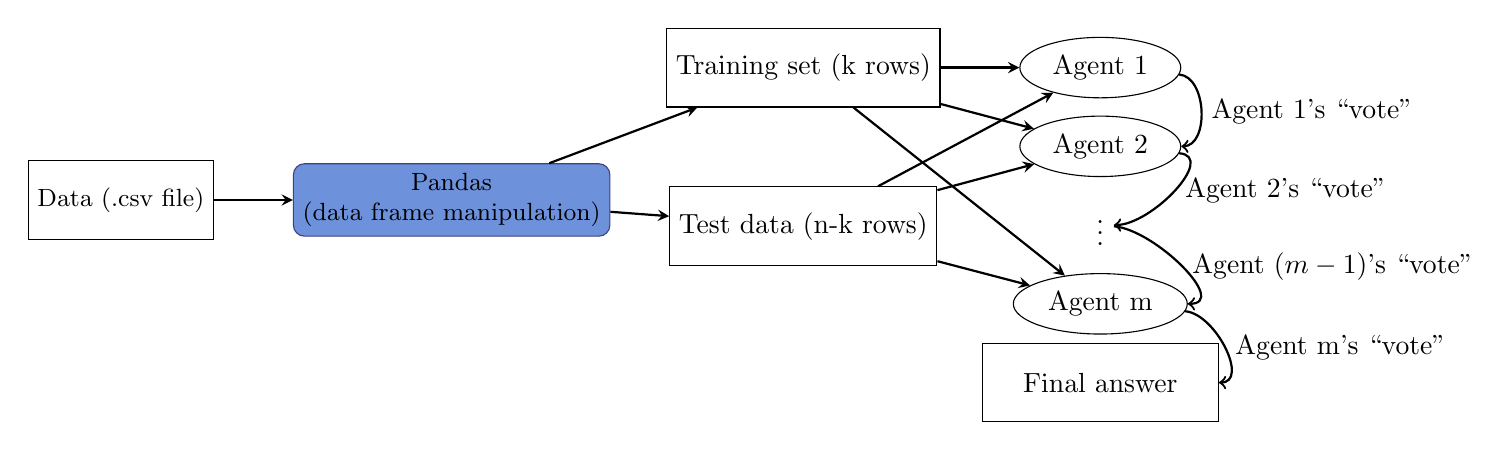
\begin{tikzpicture}[node distance=1cm, auto]
    \node (dsc) [datasrc] {Data (.csv file)};
    \node (pandas) [tool, right=1cm of dsc, align=center] {Pandas\\(data frame manipulation)};
    \node (train) [bordered, above right=1cm of pandas] {Training set (k rows)};
    %\draw [arrow] (start) -- (training);
    \node (test) [bordered, below = 1cm of train] {Test data (n-k rows)};
    \draw [arrow] (dsc) -- (pandas);
    \draw [arrow] (pandas) -- (train);
    \draw [arrow] (pandas) -- (test);
    \node (a1) [agent, right=1cm of train] {Agent 1};
    \node (a2) [agent, below of = a1] {Agent 2};
    \node (ell) [ellipsis, below of = a2,align=center] {\vdots};
    \node (a3) [agent, below of = ell] {Agent m};
    \node (fans) [bordered, below of = a3] {Final answer};
    \draw[thick,->] (a1) to[out=-5, in=0] node[right] {Agent 1's ``vote''}  (a2) ;
    \draw[thick,->] (a2) to[out=-5, in=0] node[right] {Agent 2's ``vote''}  (ell) ;
    \draw[thick,->] (ell) to[out=-5, in=0] node[right] {Agent $(m-1)$'s ``vote''}  (a3) ;
    \draw[thick,->] (a3) to[out=-5, in=0] node[right] {Agent m's ``vote''}  (fans) ;
    %\draw[thick,->] (a2) to[out=0, in=0] (ell) {Agent 2's ``vote''};
    %\draw[thick,->] (ell) to[out=0, in=0] (a3) {Agent m-1's ``vote''};
    \draw [arrow] (train) -- (a1);
    \draw [arrow] (train) -- (a2);
    \draw [arrow] (train) -- (a3);
    \draw [arrow] (test) -- (a1);
    \draw [arrow] (test) -- (a2);
    \draw [arrow] (test) -- (a3);

\end{tikzpicture}
}
\\ \\
To explain the above in more detail, the dataset (which is a csv file) will be loaded into pandas as a dataframe, where I will manipulate it to flatten out the data and break the set into the training and test sets. 
The training set will be given to each of m agents (created using the SPADE framework mentioned previously) to train a random forest classifier (taken from scikit-learn). 
Then, each row of the test set will be given to each of the agents. 
Each agent will have a randomly chosen size for their random forest; I'm currently considering the range of these to be from 5 to 20, but this range may change as experimentation progresses.
Agent 1 will use its random forest to decide what its ``vote'' is for a classification. 

Agent 1 will use SPADE's FIPA-ACL communication capabilities to convey its ``vote'' to agent 2, who will take that ``vote'' into account when making its own decision about voting for a classification of the row. 
The mechanics of how agent 2 makes a decision given agent 1's decision still need to be thought out thoroughly, but the system I envision has agent 2 finding an answer independently with its own decision tree, then comparing its answer to agent 1's answer.
If the two agents have differing answers, then agent 2 will decide between the two with probabilities weighted based on the sizes of their respective decision trees. 
For example, if agent 1 used 10 decision trees in its random forest and agent 2 used 15, then there is a 0.6 probability that agent 2 will choose its own answer, since it used a larger forest to arrive at the answer.
The voting passes on down the line in this fashion, with each agent taking into account the vote of its predecessor to inform its own decision, with the final agent (agent m) giving the final answer for the classification of the row.
\section{Algorithms Considered}
For this problem of multiagent classification, the algorithms of artificial neural networks, support vector machines, and random forest were considered. Neural networks, while flexible, have a tendency to overfit data.\textsuperscript{1}

Support vector machines are generally regarded as more performant than neural networks.\textsuperscript{1}
However, one requirement of efficiently implementing SVMs is to have an appropriate choice of kernel, which is only possible if the programmer has an intimate knowledge of the subject matter of the data.\textsuperscript{2}

A slight disadvantage of both neural networks and support vector machines is that they are black-box algorithms that lend little insight to exactly how they are making their decisions.\textsuperscript{1}

Random forest runs efficiently on large databases, can handle a high number of variables, and is generally highly accurate. Its main disadvantage is a tendency to overfit for some noisy datasets.\textsuperscript{3}

\section{Potential Pitfalls}
One aspect of this project that may cause issues is that there are 50 categories (one for each U.S. state) that the data can be classified as, which may make it difficult for the algorithm to distinguish different states from one another when they have similar metrics. For example, we may see all hospitals that perform well at treating stroke victims but poorly at treating COPD sufferers get mapped to Montana, when in fact Montana is only one of several states that have metrics that fit this pattern.
\section{Contingency Plan}
In the event that this project does not succeed as outlined, various aspects of the approach can be relaxed to increase probability of successful execution of the project. For example, the number of categories for the classification is large, so if that is found to be a difficult aspect to overcome, I can group the states into 6 distinct regions and have the algorithm predict regions rather than states. 
\section{Accomplishments Since Project Summary}
Since the submission of the project summary, I have set up a working environment which has all necessary tools installed. 
I have reviewed the tutorials and documentation for the tools I plan to use and have run a test of the random forest algorithm on the ``dummy'' dataset to ensure that random forest classifies data as I expect it to. 

I have begun learning about pandas functionality for pivoting data from being in multiple rows to multiple columns to better organize the dataset in such a way that each hospital has one row with multiple features to use for training and classifying. 
Given these accomplishments, I would consider myself on track with regard to the schedule I submitted for the initial deliverable.
At this point, I don't anticipate any major changes to the project schedule.
\section{Multiagent Communication (FIPA)}
The SPADE framework explicitly supports passing FIPA-ACL messages via the XMPP (Extensible Messaging and Presence Protocol) protocol. Since I intend to involve agent-to-agent communication in this project, I will be making use of these FIPA communication capabilities.
\section{References}
{[}1{]} Jacob Mick. (2012, June 8). Forum Post in Response to "Neural networks vs support vector machines: are the second definitely superior?" {[}Online{]}. 

Available: 
\textcolor{blue}{\underline{\href{http://stats.stackexchange.com/questions/30042/neural-networks-vs-support-vector-machines-are-the-second-definitely-superior}{http://stats.stackexchange.com/questions/30042/neural-networks-vs-support-vector-machines-}}}
\textcolor{blue}{\underline{\href{http://stats.stackexchange.com/questions/30042/neural-networks-vs-support-vector-machines-are-the-second-definitely-superior}{are-the-second-definitely-superior}}}
\\
{[}2{]} Martin Sewell. (n.d.). "Disadvantages of Support Vector Machines" {[}Online{]}. 

Available:
\textcolor{blue}{\underline{\href{http://www.svms.org/disadvantages.html}{http://www.svms.org/disadvantages.html}}}
. Accessed: Sept. 21, 2016
\\
{[}3{]} Predrag Radenkovi\'{c}. (n.d.). "Random Forest" {[}Online{]}. 

Available: 
\textcolor{blue}{\underline{\href{https://encrypted.google.com/url?sa=t\&rct=j\&q=\&esrc=s\&source=web\&cd=2\&ved=0ahUKEwiLjcO4\_qHPAhUB6CYKHa3FD6sQFgghMAE\&url=http\%3A\%2F\%2Fhome.etf.rs\%2F~vm\%2Fos\%2Fdmsw\%2FRandom\%2520Forest.pptx\&usg=AFQjCNEVo5hQOuo-6p2g3Tsa\_snZfjlNnA\&sig2=PYbl-X17PHv\_VzqJrC-pjw\&bvm=bv.133387755,d.eWE\&cad=rja}{https://encrypted.google.com/url?sa=t\&rct=j\&q=\&esrc=s\&source=web\&cd=2\&ved=0ahUK}}}
 \textcolor{blue}{\underline{\href{https://encrypted.google.com/url?sa=t\&rct=j\&q=\&esrc=s\&source=web\&cd=2\&ved=0ahUKEwiLjcO4\_qHPAhUB6CYKHa3FD6sQFgghMAE\&url=http\%3A\%2F\%2Fhome.etf.rs\%2F~vm\%2Fos\%2Fdmsw\%2FRandom\%2520Forest.pptx\&usg=AFQjCNEVo5hQOuo-6p2g3Tsa\_snZfjlNnA\&sig2=PYbl-X17PHv\_VzqJrC-pjw\&bvm=bv.133387755,d.eWE\&cad=rja}{EwiLjcO4\_qHPAhUB6CYKHa3FD6sQFgghMAE\&url=http\%3A\%2F\%2Fhome.etf.rs\%2F~vm\%2Fos\%2Fdmsw}}}
 \textcolor{blue}{\underline{\href{https://encrypted.google.com/url?sa=t\&rct=j\&q=\&esrc=s\&source=web\&cd=2\&ved=0ahUKEwiLjcO4\_qHPAhUB6CYKHa3FD6sQFgghMAE\&url=http\%3A\%2F\%2Fhome.etf.rs\%2F~vm\%2Fos\%2Fdmsw\%2FRandom\%2520Forest.pptx\&usg=AFQjCNEVo5hQOuo-6p2g3Tsa\_snZfjlNnA\&sig2=PYbl-X17PHv\_VzqJrC-pjw\&bvm=bv.133387755,d.eWE\&cad=rja}{\%2FRandom\%2520Forest.pptx\&usg=AFQjCNEVo5hQOuo-6p2g3Tsa\_snZfjlNnA\&sig2=PYbl-X17PHv\_VzqJr}}}
 \textcolor{blue}{\underline{\href{https://encrypted.google.com/url?sa=t\&rct=j\&q=\&esrc=s\&source=web\&cd=2\&ved=0ahUKEwiLjcO4\_qHPAhUB6CYKHa3FD6sQFgghMAE\&url=http\%3A\%2F\%2Fhome.etf.rs\%2F~vm\%2Fos\%2Fdmsw\%2FRandom\%2520Forest.pptx\&usg=AFQjCNEVo5hQOuo-6p2g3Tsa\_snZfjlNnA\&sig2=PYbl-X17PHv\_VzqJrC-pjw\&bvm=bv.133387755,d.eWE\&cad=rja}{C-pjw\&bvm=bv.133387755,d.eWE\&cad=rja}}}
. Accessed: Sept. 21, 2016







%Basic Format: [1] J. K. Author. (year, month day).  Title (edition) [Type of medium].  Available: http://www.(URL) 
%Example: [1] J. Jones. (1991, May 10).  Networks (2nd ed.) [Online]. Available: http://www.atm.com 

% CS 6366 Distributed AI Term Projects
% Fall 2016
% Deliverable 2
% Due: September 22, 2016 
% You are to provide an update on your project. This document is to be posted to your project web page. I will retrieve 
% it from there. Documents not posted by the start of class will be considered late and will receive a zero grade. I 
% expect this document to be less than four pages.
% This document is to contain the following items:
% 1.  Please provide any details that were requested in my feedback on your project summary.
% 2.  This deliverable is to call out specific algorithms that you intend to implement to achieve your project 
% objectives. You need to indicate what other algorithms were considered and the pros and cons of each 
% algorithm, including the chosen algorithm. Please be certain to provide appropriate references. You can use the 
% IEEE reference format: 
% http://www.ieee.org/documents/ieeecitationref.pdf. 
% Additionally, I noted on some assignments that the schedule needs to be more detailed
%  or shifted . I expect a schedule to include intermediate milestones that are between deliverable dates.  Finally, everyone is to
%  provide a contingency plan. What if you find out half way through the semester that your planned approach will not work? What will you do to ensure 
% that you have a working system appropriate for a good grade in this class by the stated deadlines?  
% 3.  Please explain what have you accomplished since the submission of the project summary?
% 4.  Where is your project as compared to the provided schedule in the project summary? If you are behind or ahead 
% of schedule, please explain why? If you are revising your schedule, please provide an updated schedule.
% 5.  What aspects of your project do you expect will change from your previous submission and why? How will you 
% address those changes? For example, if you are choosing a different algorithm, why?
% 6.  You are to provide a discussion of how the following topic relates to your project. If you have already 
% incorporated the topic into your proposal, then provide a brief review of that discussion. It is expected that you 
% will provide a well thought out discussion. If you had not planned to incorporate that specified topic into your 
% project, please discuss:
% a.  How you might incorporate the topic?
% b.  What would be the advantage of adding the topic to your project?
% c.  What would be the disadvantages of adding the topic to your project?
% d.  What would have to change about your project to incorporate the topic?

% The topic is multiple agent communication. Specifically, FIPA.
\end{document}
